\documentclass[11pt]{article}

\usepackage[margin=1in]{geometry}
\usepackage{amsmath, amssymb, amsfonts}
\usepackage{booktabs}
\usepackage{enumitem}
\usepackage{graphicx}
\usepackage{float}
\usepackage[colorlinks=true, linkcolor=blue, urlcolor=blue, citecolor=blue]{hyperref}

\graphicspath{{figures/}}

\title{First Experiment: PPO and Monte Carlo Control Against the Exact LQR Optimum}
\author{Jon Legasa}
\date{\today}

\begin{document}

\maketitle

\section*{Summary}

This is the first run of the pipeline built from the notes \emph{Measuring Reinforcement Learning
Against the Exact LQR Optimum}. Two algorithms, Proximal Policy Optimization (PPO) with a
linear-Gaussian policy and tabular first-visit Monte Carlo control, are trained on the scalar
discounted LQR problem with $\gamma = 0.99$, each on $M = 40$ seeds for $10^6$ environment steps,
and scored by the gap $g = 1 - J^*/J$ to the exact optimum. It is a \emph{crude estimate}: a small
run that produces every metric and figure of the method, not a tuned or statistically conclusive
comparison.

\begin{itemize}[leftmargin=*]
  \item PPO reaches a final mean gap of $0.0026 \pm 0.0006$ (standard error), with gain
    $0.609 \pm 0.036$ against $K^* = 0.615$. Every seed reaches $g \le 0.01$, the median seed after
    $10^5$ steps.
  \item Monte Carlo control levels off at a mean gap of about $0.72$; no seed reaches $g \le 0.1$.
  \item PPO is below Monte Carlo in every ordering of the notes from $5\times 10^4$ steps on,
    including band separation: the worst PPO seed beats the best Monte Carlo seed.
  \item For PPO the near-optimum prediction ``bias + variance'' of the notes matches the measured
    mean gap almost exactly ($0.00256$ against $0.00260$). For Monte Carlo it does not
    ($0.37$ against $0.72$), as expected far from the optimum.
\end{itemize}

%----------------------------------------------------------------------------------------------------
\section{Setup}
\label{sec:setup}

\paragraph{Problem.} The scalar system of the notes,
\[
  x_{t+1} = x_t + u_t, \qquad c(x, u) = x^2 + u^2, \qquad x_0 = 1, \qquad
  J(\pi) = \sum_{t=0}^{\infty} \gamma^t c(x_t, u_t), \qquad \gamma = 0.99 .
\]
The agents see the state and the reward $r_t = -c(x_t, u_t)$; they never see $A$, $B$, $Q$ or $R$.
There is no early termination and the dynamics are never clipped.

\paragraph{Baseline.} The discounted Riccati equation gives
\[
  K^* = 0.615251, \qquad J^* = 1.615251, \qquad c_\gamma = 1.885408,
\]
where $c_\gamma$ is the curvature of the gap at $K^*$ ($g \approx c_\gamma (k - K^*)^2$), computed
numerically as half the Hessian of the gap and equal to the closed form of the notes.

\paragraph{Score.} At each checkpoint the current policy of every seed is scored by its gap
$g = 1 - J^*/J \in [0, 1]$, with $g = 1$ when the cost is infinite.
\begin{itemize}[leftmargin=*]
  \item \textbf{PPO} is scored by its mean action $u = -kx$. The cost of a linear gain is exact (a
    Lyapunov equation), so the gap has no evaluation noise.
  \item \textbf{Monte Carlo control} is scored by its greedy policy, a lookup table, through a
    deterministic rollout of 5000 steps ($\gamma^{5000} \approx 10^{-22}$, so truncation is
    negligible). Its \emph{effective gain} is the discounted least-squares fit $u \approx -kx$
    over that rollout; it places the table on the same axis as PPO's gain.
\end{itemize}

\paragraph{Instability.} The fraction of unstable runs is reported separately from the gap, since for
$\gamma < 1$ finite cost does not imply stability. For PPO a run is unstable when
$|1 - k| \ge 1$. For Monte Carlo it is unstable when the evaluation rollout diverges or ends farther
from zero than it started (over its last 100 steps).

\paragraph{Seeds and checkpoints.} Both algorithms use the same $M = 40$ evaluation seeds, drawn
uniformly without replacement from $\{0, \dots, 2^{32}-1\}$ with master seed 0. Every random number
of a seed comes from its own generator, so a seed's run does not depend on which other seeds share
its batch (this is tested). Both are checkpointed every $5 \times 10^4$ steps, 21 checkpoints
including step 0, on the same grid, so the orderings compare the same $N$.

\paragraph{Confidence bands.} The shaded bands of the learning curves are 95\% Hoeffding bands,
simultaneous over the 21 checkpoints by the union bound:
\[
  \varepsilon = \sqrt{\frac{\ln(2 \cdot 21 / 0.05)}{2 \cdot 40}} = 0.290 .
\]
With 40 seeds the bands are wide; they are the price of a guarantee that uses only $g \in [0, 1]$.

%----------------------------------------------------------------------------------------------------
\section{Algorithms}
\label{sec:algorithms}

\subsection{PPO with a linear-Gaussian policy}

PPO follows the appendix of the notes, with a policy and value function chosen so that the optimum
can be represented exactly:
\[
  \pi_\theta(u \mid x) = \mathcal{N}(-kx,\ \sigma^2), \quad \theta = (k, \log \sigma), \qquad
  V_\phi(x) = \phi_0 + \phi_1 x + \phi_2 x^2 .
\]
The optimal policy $u = -K^* x$ is the mean of this family, and the value of a linear-Gaussian
policy on this system is exactly quadratic. The learned $k$ is therefore the gain itself, not a fit.

Each iteration collects 8 rollouts of 250 steps (2000 steps), computes advantages by generalized
advantage estimation with the discount $\gamma = 0.99$ (bootstrapping with $V$ at step 250, since
the end of a rollout is a time limit, not a terminal state), and takes 10 epochs of 4 minibatches
of gradient ascent on the combined objective
\[
  L = \hat{\mathbb{E}}\big[\min(\rho \hat A,\ \operatorname{clip}(\rho, 1-\varepsilon, 1+\varepsilon)\hat A)\big]
  - c_1 \hat{\mathbb{E}}\big[(V_\phi - \hat R)^2\big] + c_2 \hat{\mathbb{E}}\big[S[\pi_\theta]\big].
\]
The gradients are written out by hand; for this policy they are
\[
  \frac{\partial \log \pi}{\partial k} = -\frac{(u + kx)\,x}{\sigma^2}, \qquad
  \frac{\partial \log \pi}{\partial \log \sigma} = \frac{(u + kx)^2}{\sigma^2} - 1,
\]
and the gradient of the clipped term is $\rho \hat A\, \nabla \log \pi$ on samples where the
unclipped term is the minimum, and zero elsewhere. They are checked against finite differences in
the tests. The step is Adam.

\begin{table}[H]
  \centering
  \begin{tabular}{@{}llll@{}}
    \toprule
    Setting & Value & Setting & Value \\
    \midrule
    rollout length $T$ & 250 & learning rate & $3 \times 10^{-4}$ (Adam) \\
    environments per seed & 8 & GAE $\lambda$ & 0.95 \\
    epochs $E$ & 10 & clip $\varepsilon_{\mathrm{clip}}$ & 0.2 \\
    minibatches & 4 & value weight $c_1$ & 0.5 \\
    initial gain $k$ & 0 & entropy weight $c_2$ & 0 \\
    initial $\sigma$ & 0.5 & max gradient norm & 0.5 \\
    advantage normalization & per minibatch & & \\
    \bottomrule
  \end{tabular}
  \caption{PPO settings. These are common defaults, not tuned on this problem.}
\end{table}

The initial gain $k = 0$ has finite cost $J(0) = 1/(1-\gamma) = 100$, so every run starts at gap
$1 - 1.615/100 = 0.984$.

\subsection{Monte Carlo control}

On-policy first-visit Monte Carlo control with an $\varepsilon$-greedy policy (Sutton and Barto,
Section 5.4): a table $Q(s, a)$ over state bins and a fixed action grid, updated with the
sample-average step $1/n$ from the discounted return of each first visit. No bootstrapping and no
function approximation.

\begin{table}[H]
  \centering
  \begin{tabular}{@{}llll@{}}
    \toprule
    Setting & Value & Setting & Value \\
    \midrule
    state bins & 41 (odd), on $[-2, 2]$ & $\varepsilon$ & 0.1 \\
    bin spacing & $\sinh$, finer near 0 & episode length & 500 \\
    actions & 0 and $\pm$ 30 log-spaced & episodes per seed & 2000 \\
    action magnitudes & $10^{-3}$ to 2 & evaluation horizon & 5000 \\
    \bottomrule
  \end{tabular}
  \caption{Monte Carlo control settings. The odd number of bins puts one bin centred on zero.}
\end{table}

%----------------------------------------------------------------------------------------------------
\section{Results}
\label{sec:results}

\begin{table}[H]
  \centering
  \begin{tabular}{@{}lrr@{}}
    \toprule
    At $N = 10^6$ steps & Monte Carlo control & PPO \\
    \midrule
    mean gap $\pm$ SE & $0.7230 \pm 0.0352$ & $0.0026 \pm 0.0006$ \\
    95\% Hoeffding band & $[0.433, 1.000]$ & $[0.000, 0.293]$ \\
    median (IQR) & $0.795$ $(0.562\text{--}0.901)$ & $0.0017$ $(0.0004\text{--}0.0027)$ \\
    min, max over seeds & $0.270$, $0.981$ & $0.0000$, $0.0203$ \\
    floor estimate (last 10\% of checkpoints) & $0.749$ & $0.0025$ \\
    unstable fraction & $0.025$ & $0$ \\
    seeds reaching $g \le 0.1$ & 0\% & 100\% (median $5 \times 10^4$ steps) \\
    seeds reaching $g \le 0.01$ & 0\% & 100\% (median $10^5$ steps) \\
    gain, mean $\pm$ sd ($K^* = 0.615$) & $0.212 \pm 0.183$ (effective) & $0.609 \pm 0.036$ \\
    predicted gap $b^2 c_\gamma + c_\gamma s^2$ & $0.307 + 0.063 = 0.370$ & $0.00008 + 0.00248 = 0.00256$ \\
    median $|x|$ after evaluation & $0.175$ & --- \\
    wall time (20 processes) & 37 s & 10 s \\
    \bottomrule
  \end{tabular}
  \caption{Headline numbers at the final checkpoint, $M = 40$ seeds each.}
  \label{tab:results}
\end{table}

\paragraph{Orderings.} With PPO as $A$ and Monte Carlo as $B$, on identical checkpoints:
\begin{center}
  \begin{tabular}{@{}lcc@{}}
    \toprule
    Ordering & holds at $N = 10^6$ & holds from \\
    \midrule
    band separation ($\max_\omega g_A \le \min_{\omega'} g_B$) & yes & $5 \times 10^4$ \\
    expected curves ($\hat g_A \le \hat g_B$) & yes & $0$ \\
    confident (upper band of $A$ below lower band of $B$) & yes & $5 \times 10^4$ \\
    floors & yes & --- \\
    \bottomrule
  \end{tabular}
\end{center}
At $N = 0$ both algorithms start near gap 1 and the bands overlap; from the first checkpoint on, the
ordering holds in every sense.

%----------------------------------------------------------------------------------------------------
\section{Figures}
\label{sec:figures}

\subsection{Both algorithms}

\begin{figure}[H]
  \centering
  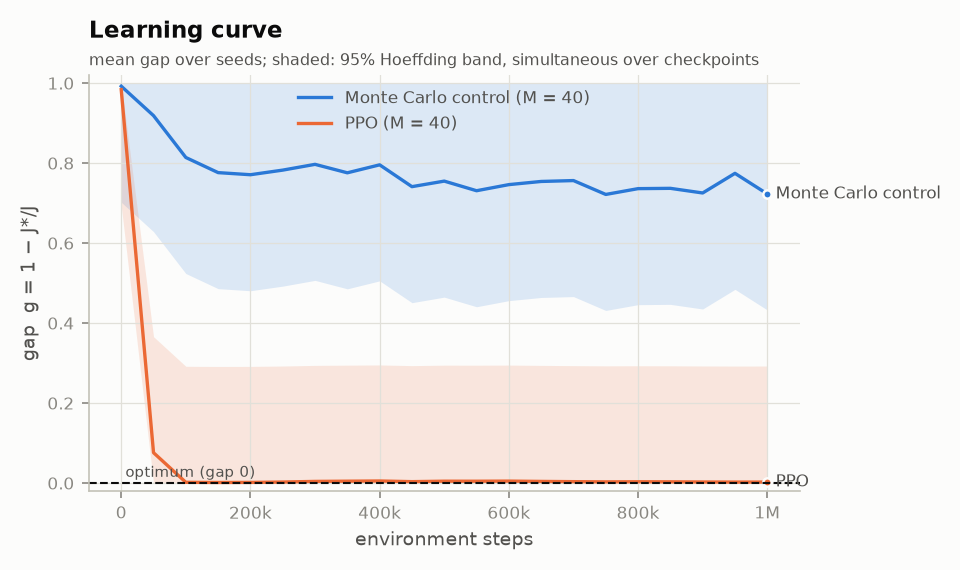
\includegraphics[width=0.85\textwidth]{learning_curves.png}
  \caption{\textbf{Learning curves.} The mean gap $\hat g(N)$ over the 40 seeds of each algorithm
    against environment steps, with the shaded 95\% Hoeffding band, simultaneous over the 21
    checkpoints (half-width 0.29). The dashed line at zero is the optimum. PPO falls from 0.98 to
    below 0.01 within $10^5$ steps; Monte Carlo control falls to about 0.8 by $1.5 \times 10^5$
    steps and then stays between 0.72 and 0.80. The two bands separate from the first checkpoint
    on. The PPO band reaches up to 0.29 only because Hoeffding uses nothing but $g \in [0, 1]$; its
    seeds are far more concentrated than that (Figure~\ref{fig:ppo-runs}).}
  \label{fig:curves}
\end{figure}

\begin{figure}[H]
  \centering
  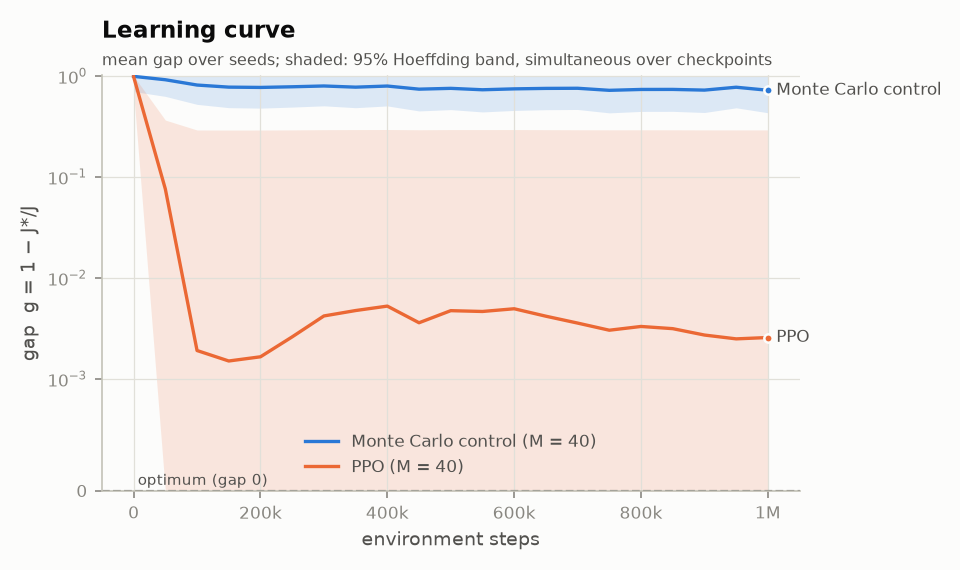
\includegraphics[width=0.85\textwidth]{learning_curves_log.png}
  \caption{\textbf{Learning curves, logarithmic gap axis.} The same curves on a symmetric-log axis
    (linear near zero), to show what the linear axis hides near the optimum. PPO's mean gap
    reaches about $1.6 \times 10^{-3}$ at $1.5 \times 10^5$ steps, then rises to about
    $5 \times 10^{-3}$ around $4 \times 10^5$ steps and drifts back down to $2.6 \times 10^{-3}$.
    It does not keep decreasing: the exploration noise $\sigma$ has collapsed, so the gains stop
    moving (Section~\ref{sec:observations}). Monte Carlo control stays within a factor 1.4 of
    gap 1 throughout.}
  \label{fig:curves-log}
\end{figure}

\begin{figure}[H]
  \centering
  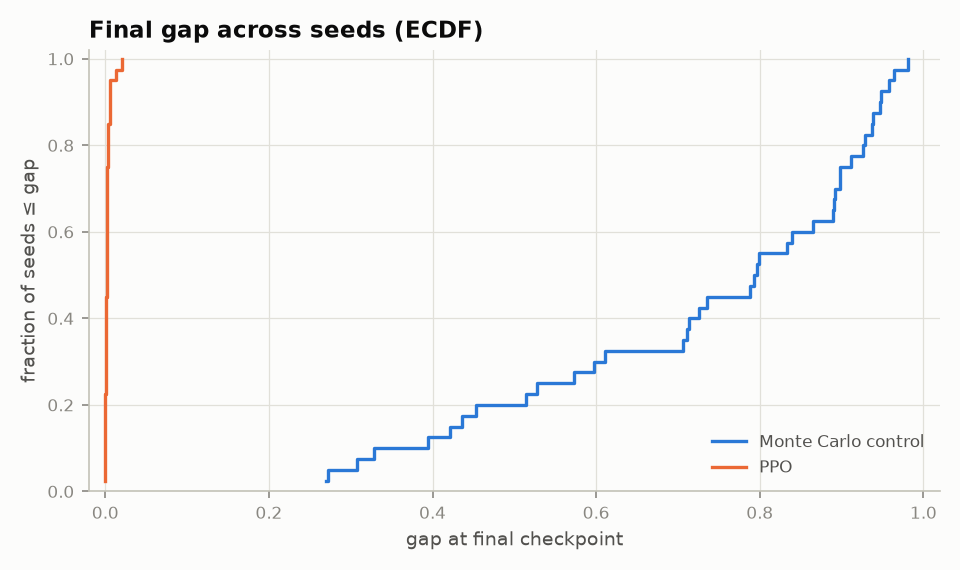
\includegraphics[width=0.85\textwidth]{final_gap_ecdf.png}
  \caption{\textbf{Distribution of the final gap across seeds.} Empirical cumulative distribution
    of $g(\omega, 10^6)$: the height at gap $x$ is the fraction of seeds with final gap at most
    $x$. All PPO seeds lie below 0.021; the Monte Carlo seeds spread from 0.27 to 0.98, with half
    of them above 0.79. The two distributions do not overlap, which is band separation at the
    final checkpoint.}
  \label{fig:ecdf}
\end{figure}

\begin{figure}[H]
  \centering
  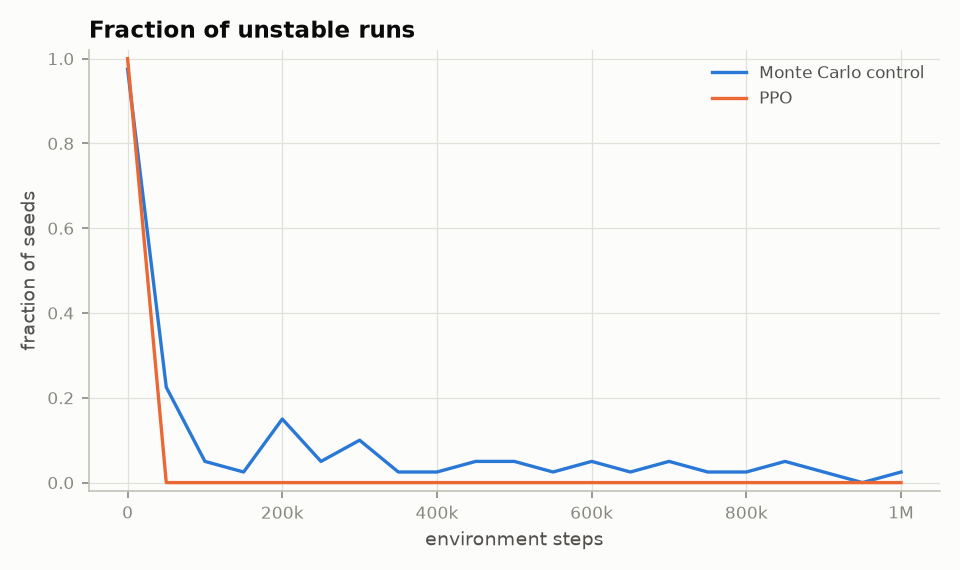
\includegraphics[width=0.85\textwidth]{unstable_fraction.png}
  \caption{\textbf{Fraction of unstable runs.} The fraction of seeds whose current policy is
    unstable, reported separately from the gap because finite discounted cost does not imply
    stability. At step 0 both are (marginally) unstable: PPO starts at $k = 0$, for which
    $|1 - k| = 1$, and the untrained Monte Carlo table drifts away from zero. PPO is stable on every
    seed from the first checkpoint on. Monte Carlo keeps 0--15\% of seeds unstable, i.e.\ ending the
    evaluation rollout farther from zero than $x_0 = 1$; 1 of the 40 seeds (2.5\%) at the end.}
  \label{fig:unstable}
\end{figure}

\subsection{PPO}

\begin{figure}[H]
  \centering
  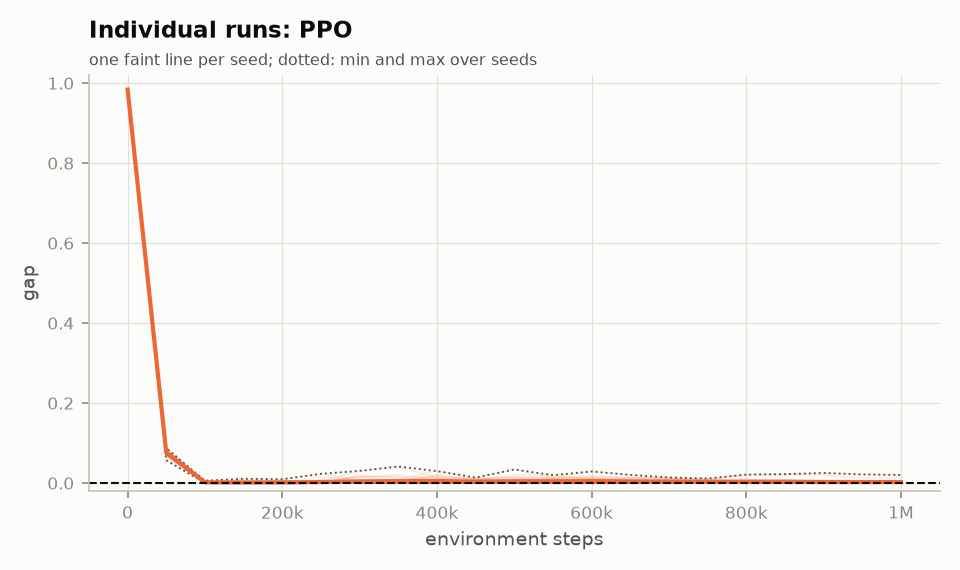
\includegraphics[width=0.85\textwidth]{ppo_runs.png}
  \caption{\textbf{Individual PPO runs.} One faint line per seed, the mean in bold, and the minimum
    and maximum over seeds dotted. The 40 runs are almost indistinguishable: all of them drop below
    gap 0.1 by $5 \times 10^4$ steps, and the worst seed stays below 0.04 after that. This is
    the envelope used for band separation.}
  \label{fig:ppo-runs}
\end{figure}

\begin{figure}[H]
  \centering
  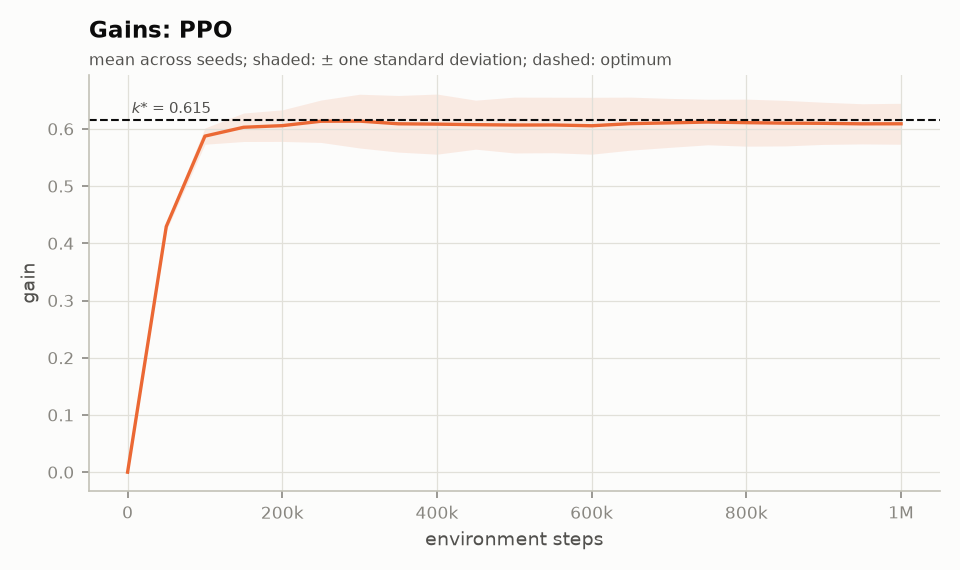
\includegraphics[width=0.85\textwidth]{ppo_gains.png}
  \caption{\textbf{PPO gains.} The mean learned gain $k$ across seeds, shaded $\pm$ one standard
    deviation, against the optimum $K^* = 0.615$ (dashed). The mean reaches 0.59 at $10^5$ steps
    and sits at $0.61$ from $1.5 \times 10^5$ steps on, so the bias is small. The spread across
    seeds, about $\pm 0.04$, does not shrink: once $\sigma$ has collapsed each seed keeps the gain
    it had. Because the policy is linear this is the gain itself, not a fit.}
  \label{fig:ppo-gains}
\end{figure}

\begin{figure}[H]
  \centering
  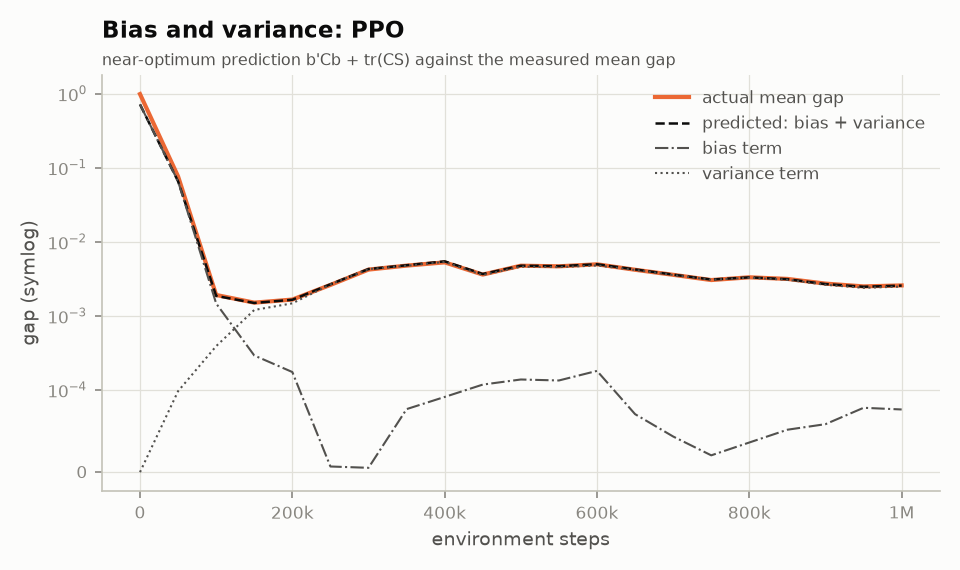
\includegraphics[width=0.85\textwidth]{ppo_bias_variance.png}
  \caption{\textbf{PPO: bias and variance of the gain against the gap.} The measured mean gap
    (solid) and the near-optimum prediction of the notes,
    $\bar g \approx c_\gamma\,(\text{bias}^2 + \text{variance})$ (dashed), with its bias term
    $c_\gamma (\bar k - K^*)^2$ (dash-dot) and variance term $c_\gamma s_k^2$ (dotted), on a
    symmetric-log axis. After the first $10^5$ steps the prediction and the measurement coincide.
    Early on the gap is bias (the gains have not reached $K^*$); from about $1.5 \times 10^5$ steps
    the variance term dominates by one to two orders of magnitude: the remaining gap is almost
    entirely spread across seeds, not a systematic error.}
  \label{fig:ppo-bv}
\end{figure}

\begin{figure}[H]
  \centering
  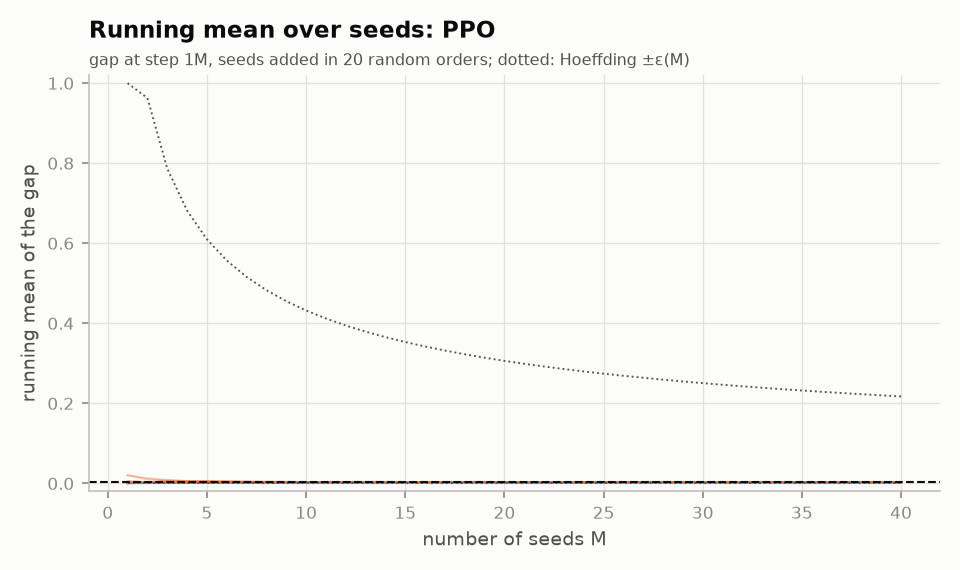
\includegraphics[width=0.85\textwidth]{ppo_running_means.png}
  \caption{\textbf{PPO: running mean over seeds (strong law of large numbers).} The final gaps are
    averaged over the first $1, 2, \dots, 40$ seeds, in 20 random orders of the seeds; each line
    is one sample path of the estimator $\hat g$ as seeds are added. The dashed line is the mean
    over all 40, and the dotted line is the Hoeffding half-width $\varepsilon(M)$ around it (cut
    at 0 and 1). The paths are already flat at about 0.003 after a few seeds, far inside the
    Hoeffding envelope, because the PPO gaps vary much less than the worst case
    $\mathrm{Var} \le 1/4$ that Hoeffding allows for.}
  \label{fig:ppo-running}
\end{figure}

\subsection{Monte Carlo control}

\begin{figure}[H]
  \centering
  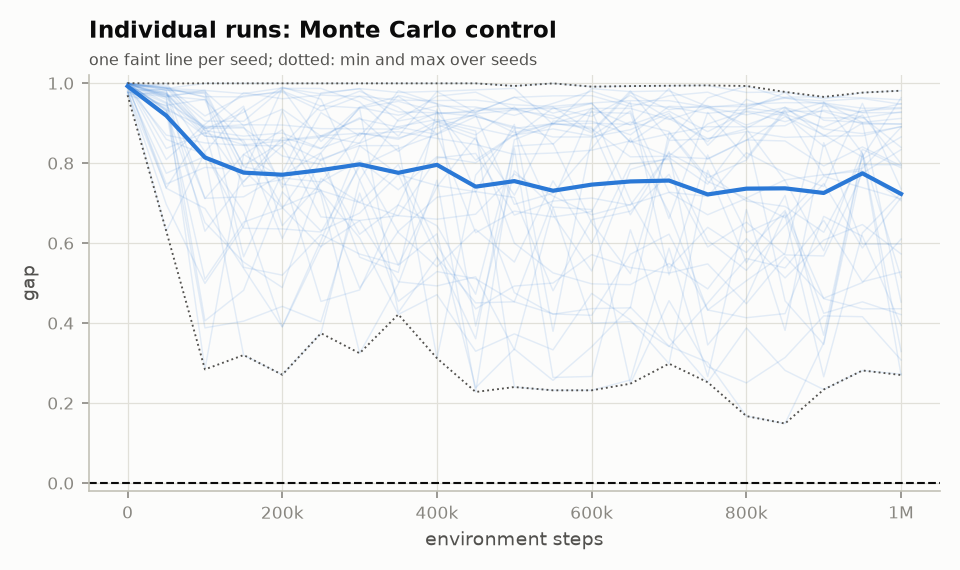
\includegraphics[width=0.85\textwidth]{monte_carlo_runs.png}
  \caption{\textbf{Individual Monte Carlo control runs.} One faint line per seed, the mean in bold,
    the minimum and maximum over seeds dotted. Individual runs jump by several tenths from one
    checkpoint to the next: the greedy policy of a table changes discretely as the estimates of
    $Q$ cross each other. The best seed at any checkpoint is between 0.15 and 0.4, the worst
    near 1. The runs do not settle.}
  \label{fig:mc-runs}
\end{figure}

\begin{figure}[H]
  \centering
  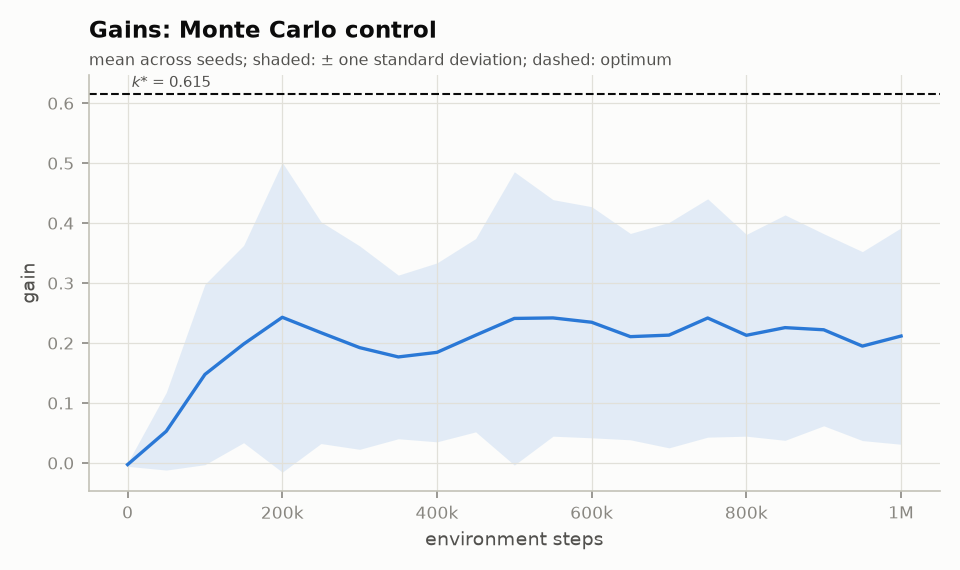
\includegraphics[width=0.85\textwidth]{monte_carlo_gains.png}
  \caption{\textbf{Monte Carlo control effective gains.} The mean effective gain, the discounted
    least-squares fit $u \approx -kx$ of the greedy table along its evaluation rollout, shaded
    $\pm$ one standard deviation, against $K^* = 0.615$. The mean rises to about 0.2 by
    $2 \times 10^5$ steps and stays there; the spread across seeds is about $\pm 0.18$. The table
    acts much more weakly than the optimal controller, which matches the residual state of
    Figure~\ref{fig:mc-residual}.}
  \label{fig:mc-gains}
\end{figure}

\begin{figure}[H]
  \centering
  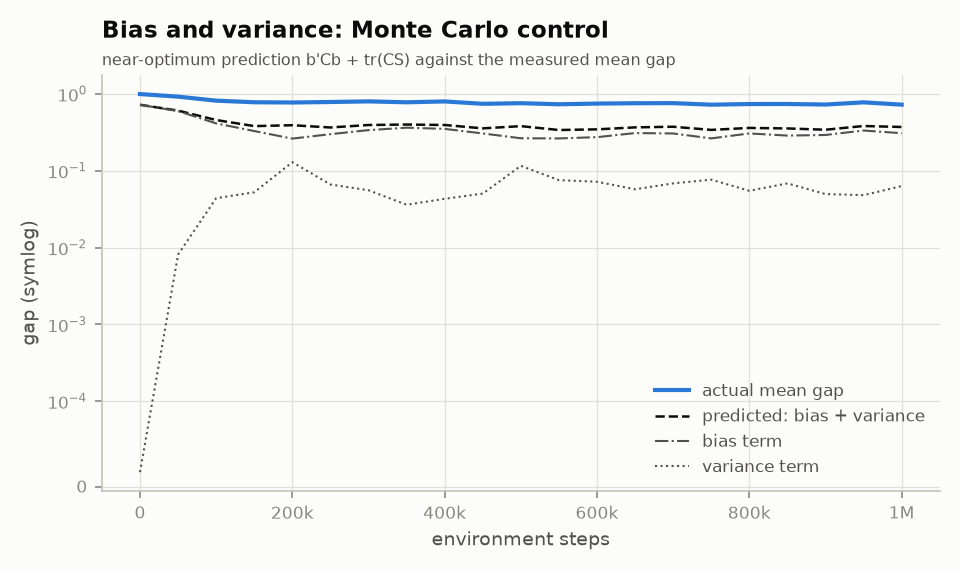
\includegraphics[width=0.85\textwidth]{monte_carlo_bias_variance.png}
  \caption{\textbf{Monte Carlo control: bias and variance against the gap.} As in
    Figure~\ref{fig:ppo-bv}, with the effective gain. The prediction (dashed, about 0.37 at the
    end) is roughly half the measured gap (solid, 0.72), and the bias term dominates the variance
    term by a factor of about 5. The approximation $g \approx c_\gamma e^2$ holds only near $K^*$,
    and the table is neither near $K^*$ nor linear, so the effective gain does not capture its
    cost: this is the ``locality'' limitation of the notes, visible in data.}
  \label{fig:mc-bv}
\end{figure}

\begin{figure}[H]
  \centering
  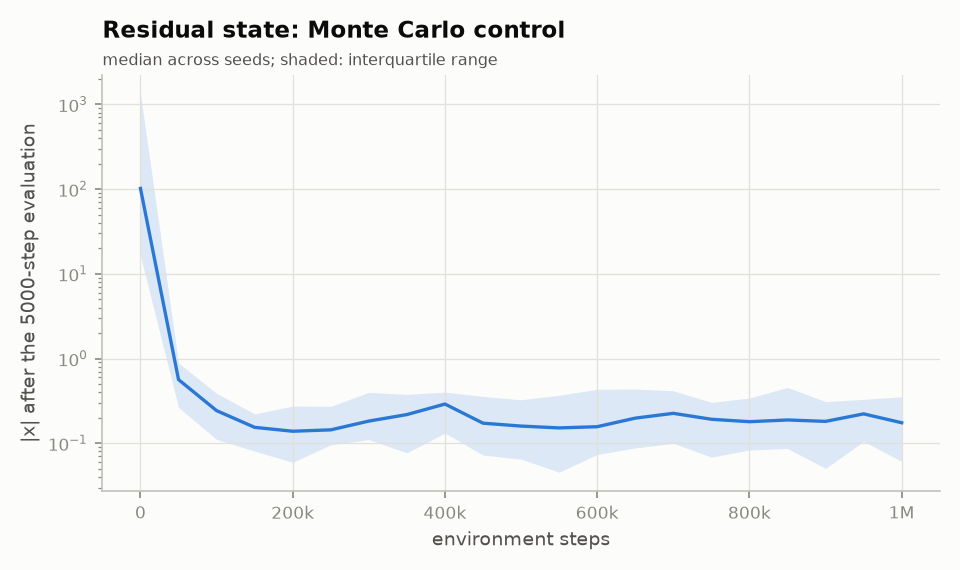
\includegraphics[width=0.85\textwidth]{monte_carlo_residual_state.png}
  \caption{\textbf{Monte Carlo control: residual state.} The median over seeds of $|x|$ at the end
    of the 5000-step evaluation rollout of the greedy table, shaded by the interquartile range, on
    a log axis. The untrained table drifts to $|x| \approx 100$. After training, the state stops at
    $|x| \approx 0.15$--$0.3$ and never reaches zero: near zero the table's greedy action does not
    push the state further. A state stuck at $|x|$ costs $x^2/(1-\gamma) = 100x^2$, so
    $|x| \approx 0.175$ alone adds about 3 to $J^* = 1.6$, enough to explain most of the gap.}
  \label{fig:mc-residual}
\end{figure}

\begin{figure}[H]
  \centering
  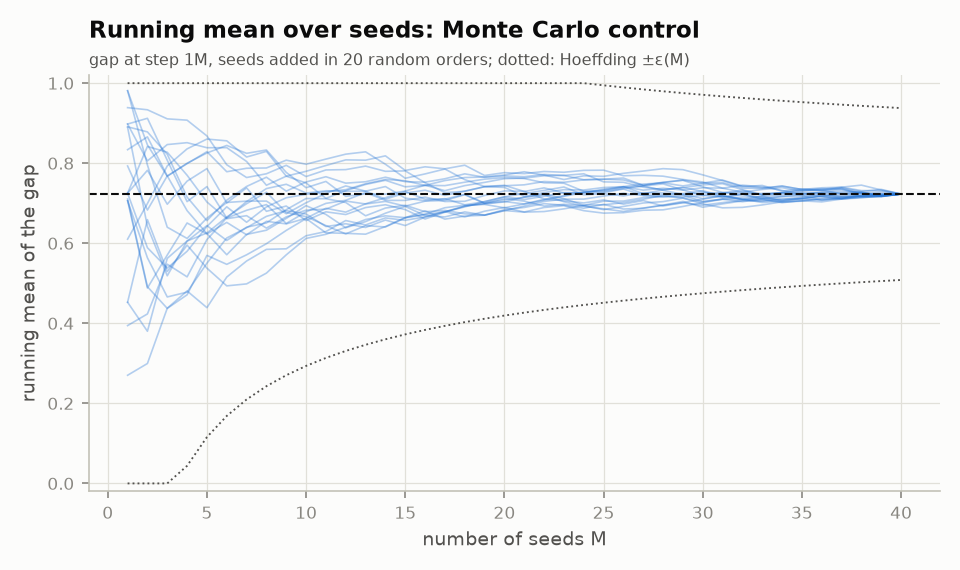
\includegraphics[width=0.85\textwidth]{monte_carlo_running_means.png}
  \caption{\textbf{Monte Carlo control: running mean over seeds (strong law of large numbers).} As in
    Figure~\ref{fig:ppo-running}. With few seeds the running mean ranges from 0.27 to 0.98,
    depending on which seeds come first; by 20 seeds the 20 paths agree to within about
    $\pm 0.05$, and they meet at 0.72 at 40 seeds by construction. The paths stay inside the
    Hoeffding envelope, which is still $\pm 0.21$ wide at $M = 40$ for a single checkpoint.}
  \label{fig:mc-running}
\end{figure}

%----------------------------------------------------------------------------------------------------
\section{Observations}
\label{sec:observations}

\paragraph{PPO's exploration collapses.} With no entropy bonus ($c_2 = 0$), the median $\sigma$ across
seeds falls from 0.5 to 0.19 at $10^5$ steps, 0.08 at $2 \times 10^5$ and 0.005 at $10^6$. Once $\sigma$ is small the data carry almost no information about
$k$, so each seed's gain stays where it is. This explains why the PPO curve stops decreasing at a
gap of a few $10^{-3}$ and why its variance term dominates (Figure~\ref{fig:ppo-bv}). In a probe
with 8 seeds and a learning rate ten times larger ($3 \times 10^{-3}$), $\sigma$ collapsed within
$2 \times 10^5$ steps and the mean gap stayed at about 0.02. The floor of PPO here is set by its
exploration, not by its policy class, which contains the optimum.

\paragraph{The final PPO gap is noisy at this scale.} An earlier run with rollouts of 200 instead of
250 steps ended at a mean gap of 0.0002 rather than 0.0026, with the same plateau of 0.002--0.005
along the way. The last checkpoint alone should be read as ``of order $10^{-3}$''; the floor
estimate over the last checkpoints is the more stable number.

\paragraph{Monte Carlo control stalls at a residual state.} The hypothesis, not yet tested, is that
with $\varepsilon = 0.1$ and random actions up to $\pm 2$, the return following an action near
$x = 0$ is dominated by the cost of later random actions, so the small differences between good
actions there are lost in the noise, and the greedy choice near zero is close to arbitrary.

\paragraph{The bias--variance split works where the notes say it should.} Near the optimum (PPO)
$\bar g \approx c_\gamma(\text{bias}^2 + \text{variance})$ is accurate to about 2\%; far from it
(Monte Carlo) it is off by a factor of two.

%----------------------------------------------------------------------------------------------------
\section{Limitations of this run}

\begin{itemize}[leftmargin=*]
  \item \textbf{40 seeds.} The simultaneous Hoeffding bands have half-width 0.29. The ordering is
    conclusive here only because the gap between the algorithms is so large; to resolve
    differences of a few hundredths, the notes' budget asks for about 1000--1300 seeds.
  \item \textbf{No tuning.} Both algorithms use default settings. The notes prescribe tuning on
    separate seeds before the evaluation seeds; this run has no tuning seeds.
  \item \textbf{One problem.} Only the scalar LQR. LQI (the two-dimensional augmented system) is
    supported by the code but not yet run.
  \item \textbf{Different evaluation of the two algorithms.} PPO's gap is exact for its mean
    action; Monte Carlo's comes from a 5000-step rollout of its greedy table. Both are
    deterministic, and the truncation error of the rollout is of order $10^{-22}$.
\end{itemize}

%----------------------------------------------------------------------------------------------------
\section{Reproducing}

From the repository root:
\begin{verbatim}
uv run main.py baseline --problem lqr --gamma 0.99
uv run main.py crude --algos monte_carlo ppo --problem lqr
\end{verbatim}
The run reported here is \texttt{results/crude\_20261116-004618\_lqr/}, with master seed 0, 40 seeds
per algorithm and 20 worker processes; a seed's result does not depend on the number of workers.
The figures in \texttt{figures/} are copied from its \texttt{report/} directory.

\end{document}
